\section{Practical Example}


To accompany this project, we developed a Plugin for the Minecraft Spigot Server software, that constructs a MCWATER world for a given CNF formula and brute-forces all possible water assignments. The code and binaries can be found in this \href{https://github.com/JonathanDotExe/minecraft-water-problem}{GitHub repository}. A video demonstration of the plugin can be found \href{https://youtube.com}{here}.

\emph{Disclaimer: } Technically this implementation is not exactly equal to our described problem, because we did some abstractions, to prevent complex interactions between the environment/player and our construction. This plugin does also not generate an entire word, but places the machine encoding a CNF formula into an existing world. Still, if the player and any non-player characters don't interfere with the machine, it works like it does in our abstraction and nicely illustrates our project.

\paragraph{Installation}
A brief tutorial on how to setup a Spigot Server and install a plugin (our plugin .jar can be found in the linked GitHub repository) can be found \href{https://www.spigotmc.org/wiki/spigot-installation/}{here}.

\paragraph{Usage}
To generate a structure, a player with operator privileges simply has to enter the following command: \verb|/generatecnf <formula>|. In our syntax $\&$ represents $\wedge$, $\vert$ represents $\vee$ and ! represents $\neg$. For example $(x | y) \& (!x)$ would mean $(x \vee y) \wedge (\neg \; x)$.

\begin{figure}[h]
    \centering
    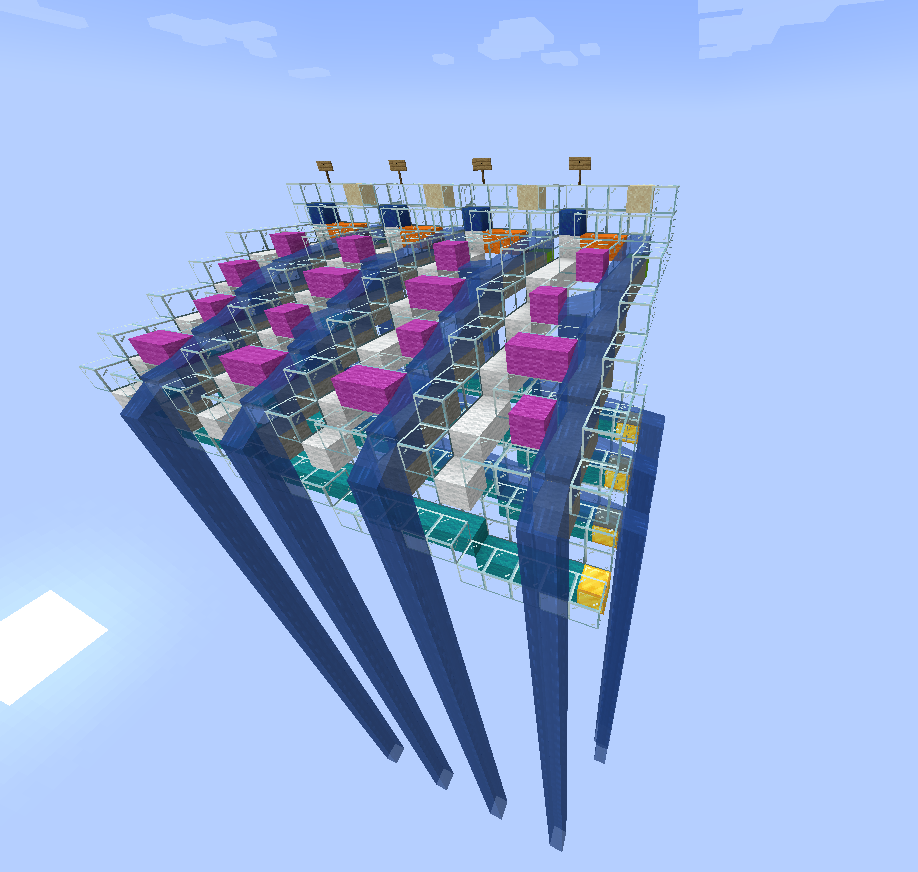
\includegraphics[width=.5\linewidth]{images/big_example.png}
    \cprotect\caption{The structure generated for \verb+/generatecnf (a | !b | !c | d) & (!a | !d) & (!b | c | d) & (a)+}
    \label{fig:small-example}
\end{figure}

